\section{Introduction}

Building general-purpose embodied agents requires policies that can not only map visual observations to actions, but also reason about how the physical world evolves under interaction. This has motivated growing interest in World Action Models (WAMs), which combine future visual prediction and action modeling in a unified framework. Compared with standard Vision-Language-Action (VLA) models, WAMs are appealing because modeling future observations may help capture physical dynamics and task-relevant temporal structure.

Most existing WAMs follow an imagine-then-execute paradigm: they first generate future observations, then predict actions conditioned on the imagined future. While intuitive, this design incurs substantial test-time latency due to iterative video denoising~\cite{pai2025mimicvideo,liang2025videogenerators,lingbot-va2026, ye2026worldactionmodelszeroshot, bi2025motusunifiedlatentaction}. More fundamentally, it remains unclear whether explicit future imagination is actually necessary for strong action performance. The effectiveness of WAMs may stem from two distinct sources: \emph{(1)} the video prediction objective during training, which may help the model acquire stronger physical priors and action-conditioned representations, and \emph{(2)} explicit future generation during inference, which may provide additional foresight for action prediction. Existing WAM systems typically entangle these two factors, making it difficult to determine which one is actually responsible for the observed gains.

In this paper, we revisit this design choice and ask a simple question: \emph{do WAMs need to imagine future observations at test time, or do they benefit primarily from learning to model them during training?} Our key idea is to decouple the video prediction objective used in WAM training from explicit future generation at inference time. If the main value of world modeling lies in shaping better latent representations during training, then a WAM should be able to retain this benefit without paying the test-time cost of future video synthesis.

\begin{figure*}[tbp]
        \centering
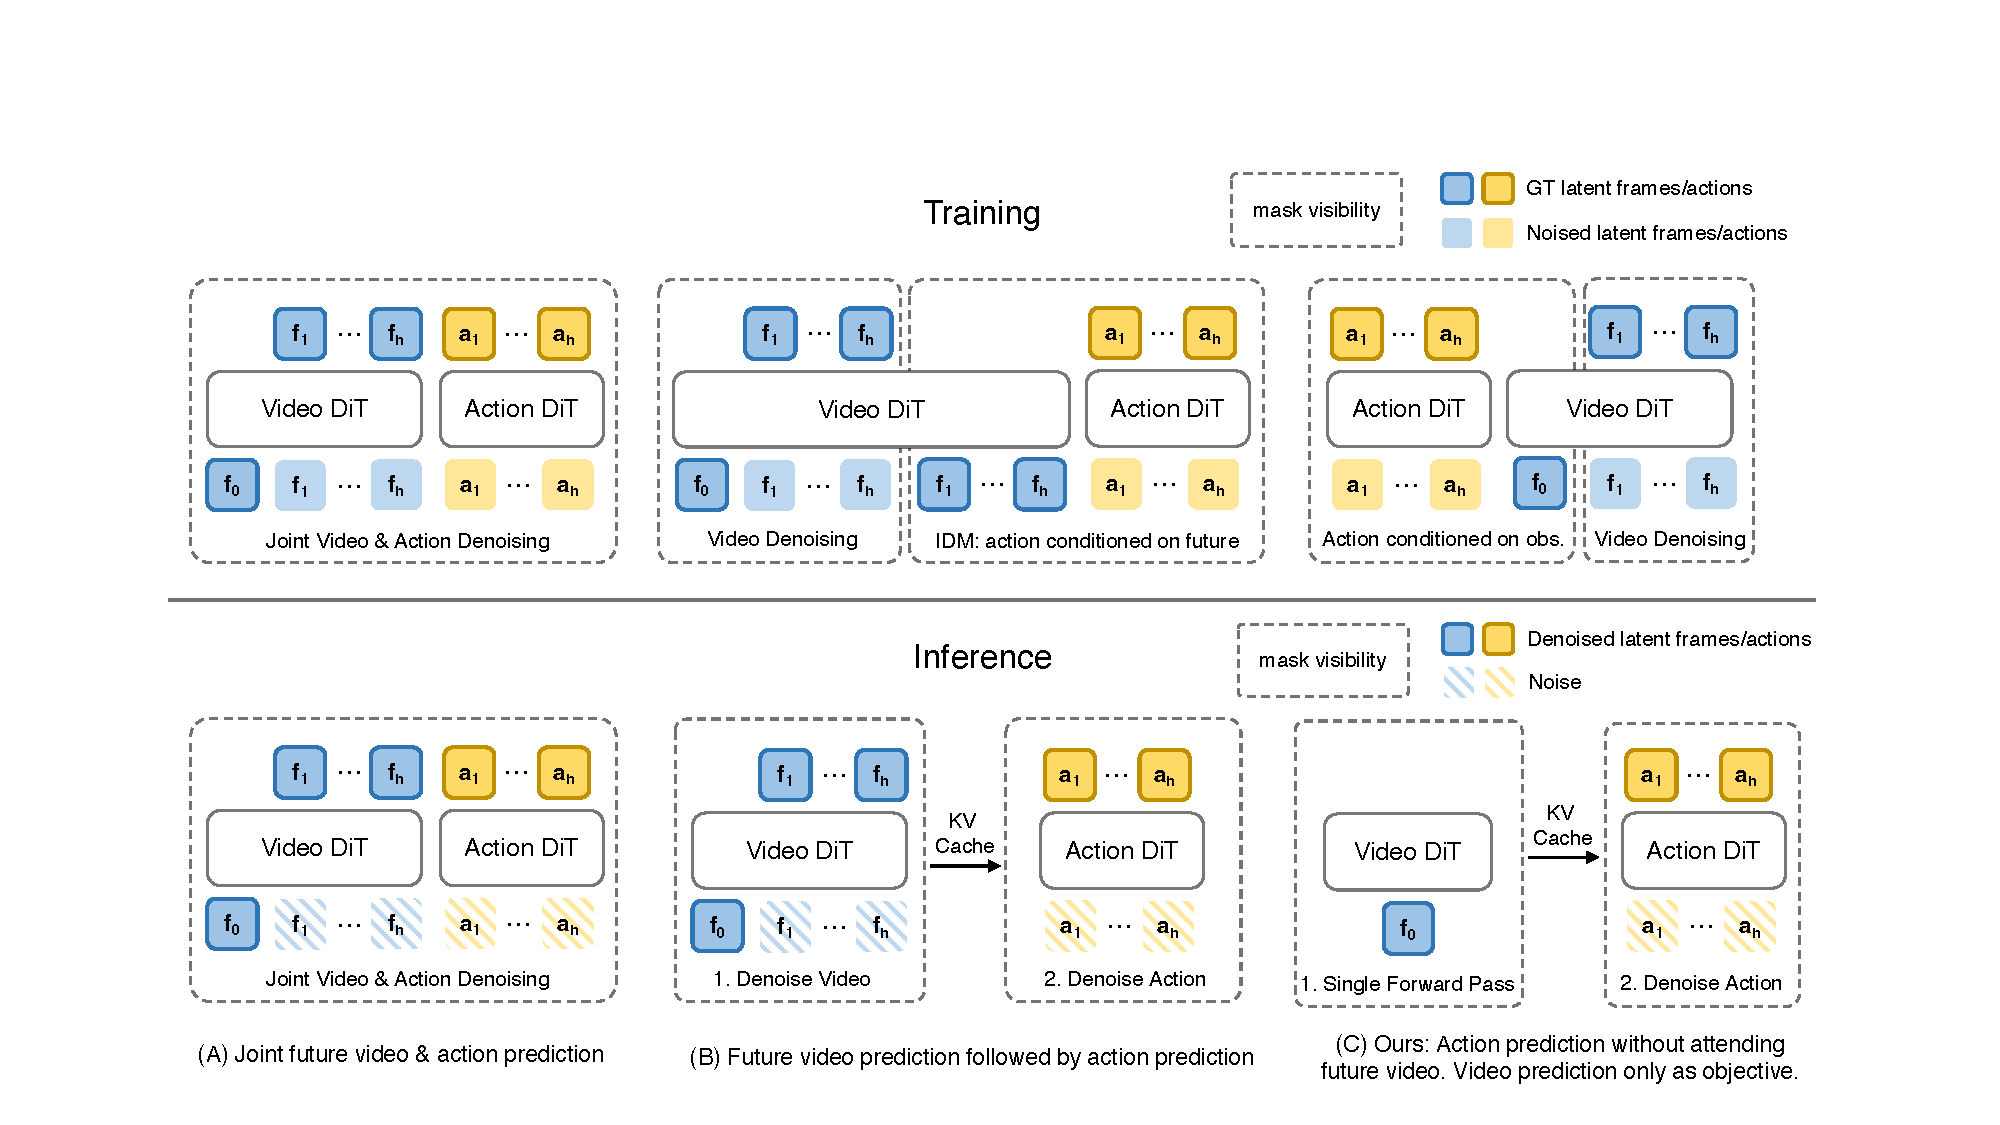
\includegraphics[width=1.0\textwidth]{figs/teaser_main_new.pdf} 
    \caption{Three representative WAM paradigms. (A) Joint-modeling WAMs denoise future video and action tokens together. (B) Causal WAMs first generate future observations and then condition action prediction on the generated future representation. (C) Fast-WAM retains video co-training during training but removes explicit future generation at inference time, directly predicting actions from latent world representations in a single forward pass.}
    \label{fig:three_types}
\end{figure*}

Based on this perspective, we propose \textbf{Fast-WAM}, a WAM architecture that preserves video co-training during training but skips future prediction at test time. Instead of using a pretrained video generation model to iteratively synthesize future frames during inference, Fast-WAM repurposes a pretrained video Diffusion Transformer (DiT) as a single-pass world encoder for action generation. Concretely, we build Fast-WAM with a Mixture-of-Transformer (MoT) architecture with shared attention, consisting of a video DiT and an action expert DiT, as illustrated in Figure~\ref{fig:three_types}(C). During training, the video prediction objective shapes the video DiT to encode physically meaningful motion and interaction structure. During inference, the video DiT processes the observation context in a single forward pass and provides latent world representations for action denoising, avoiding explicit future video denoising and enabling efficient real-time control.

To study our central question in a controlled way, we instantiate Fast-WAM into variants that mirror representative imagine-then-execute WAM designs. For simplicity, we focus on single action chunk generation and omit the outer auto-regressive loop. As shown in Figure~\ref{fig:three_types}, existing WAMs can be broadly grouped into two representative paradigms: \emph{(A)} future videos and actions are jointly denoised with shared attention~\cite{ye2026worldactionmodelszeroshot, zhu2025unifiedworldmodelscoupling, bi2025motusunifiedlatentaction}; and \emph{(B)} actions are predicted after, and conditioned on, generated future videos~\cite{lingbot-va2026, feng2025vidarembodiedvideodiffusion, du2023learninguniversalpoliciestextguided}. We also implement a no-video-co-training variant, which serves as a direct control for the role of the training objective itself. Together, these controlled comparisons allow us to isolate the contribution of test-time future imagination from that of video co-training during training.

Experiments on simulation benchmarks (LIBERO and RoboTwin) show that Fast-WAM achieves strong results without any embodied pretraining, demonstrating strong data efficiency. On real-world robotic tasks, Fast-WAM remains highly effective while running at only 190\,ms latency, making it more than 4$\times$ faster than existing imagine-then-execute WAM approaches. More importantly, controlled comparisons show that Fast-WAM stays close to imagine-then-execute variants, while removing the video co-training objective causes a much larger performance drop. These results suggest that the main value of video prediction in WAMs may lie in improving world representations during training rather than in explicitly generating future observations at test time.

Our contributions are three-fold:
\begin{itemize}
    \item We identify and study a basic question in WAMs: whether their gains come primarily from video modeling during training or from explicit future imagination during inference.
    \item We propose Fast-WAM, a WAM architecture that retains video co-training during training while eliminating future prediction at test time, enabling real-time inference.
    \item Through controlled comparisons on simulation and real-world benchmarks, including variants with and without video co-training, we show that much of the benefit of WAMs comes from the video co-training objective itself, while explicit future generation at inference time appears to be less critical than previously assumed.
\end{itemize}
